\exercise{Slow-Fast}{3}
Analyze the following system 
\eqan{
\dot{x}&=&-x^3+x+y \\
\dot{y}&=&-\alpha x
}
where again $\alpha\ll 1$. What happens in this system in the long run? (Hint: Make sure to check the stability of the slow manifold, the result may be surprising)

\solution
In this case the fast dynamics is 
\eq{
\dot{x}=-x^3+x+y 
}
we solve for the steady state
\eqa{
0&=&-x^3+x+y \\
y&=&x^3-x 
}
Note that in the fast dynamics $y$ only appears as a parameter 
rather then a variable. So normally we would solve for $x(y)$ rather than $y(x)$ but the third root makes this quite horrible. But already the solution in the form $y(x)$ allows us to draw the solution branches.

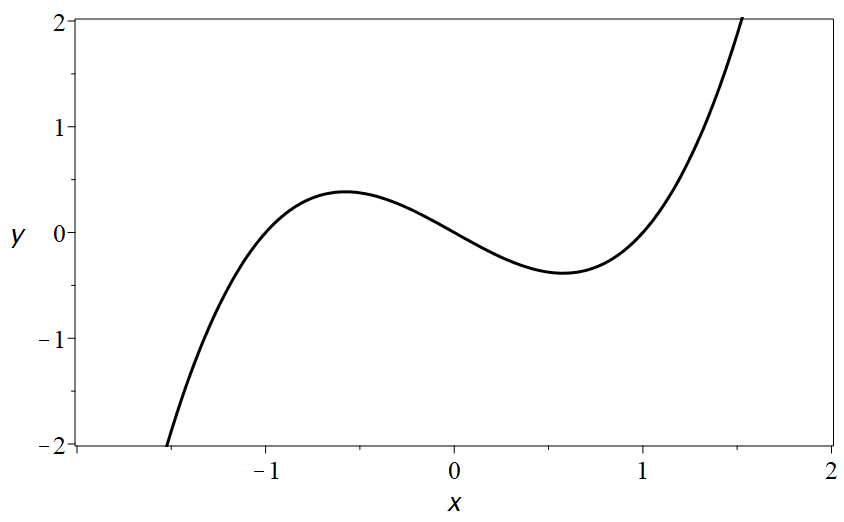
\includegraphics[width=0.8\textwidth]{slowfastcycle1}

Is this slow manifold stable? Or rather, which parts of it are stable? 
To check the stability mathematically we need the Jacobian
\eq{
{\bf J}= \frac{\partial \dot{x}}{\partial x} = -3x^2+1 
}
Even without knowing the steady states, we know that stability requires
\eq{
0 > -3x^2+1 
}
in the steady state. We find the bifurcations by solving 
\eqa{
0 &=& -3x^2+1  \\
x &=& \pm \sqrt{\frac{1}{3}} 
}
So we can see that the slow manifold is unstable for $\sqrt{-1/3}\leq x \leq \sqrt{1/3}$ and stable otherwise. Let's plot that.

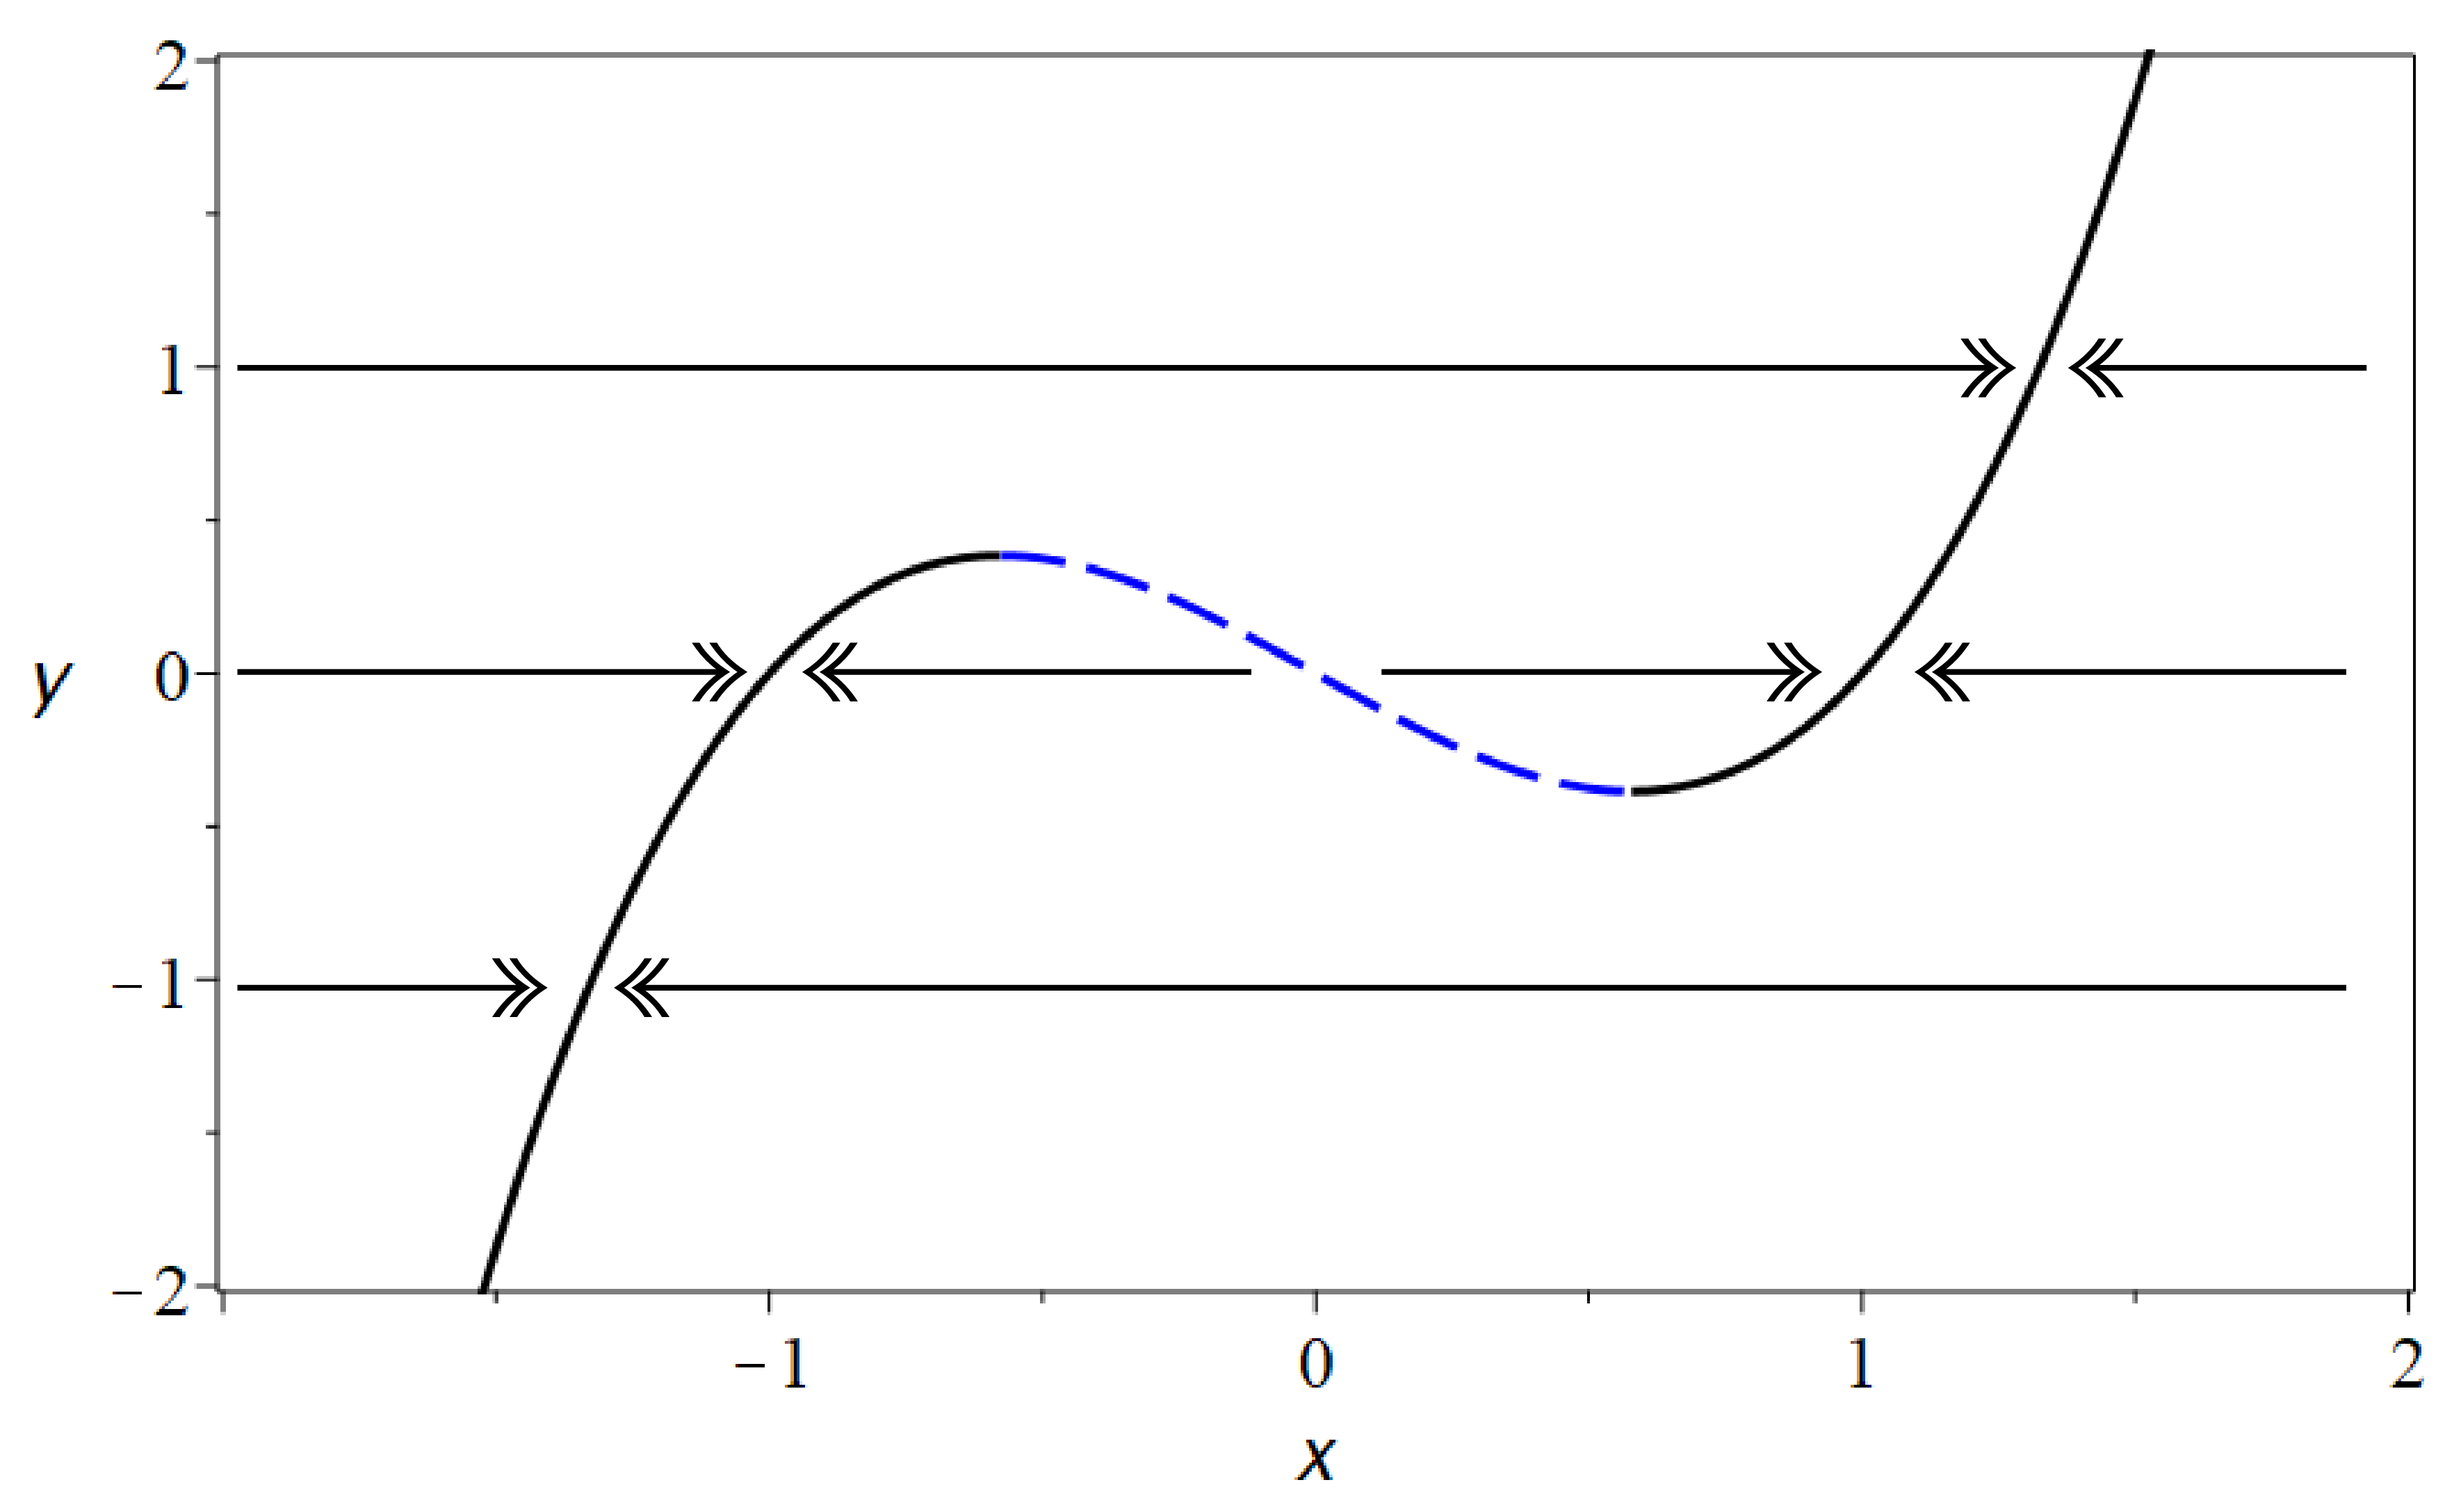
\includegraphics[width=0.8\textwidth]{slowfastcycle2}

Now we also have to consider the slow dynamics. This follows
\eq{
\dot{y}=-\alpha x
}
Because $\alpha>0$ this means that $y$ will slowly increase if $x<0$ and $y$ will slowly decrease if $x>0$.\nl

So if we are on the stable branch of the slow manifold at $x>0$ we move slowly downwards along the manifold until we hit the fold bifurcation. \nl

At this point our branch of the slow manifold is destroyed, so fast dynamics sets in and takes us rapidly to the other branch. \nl

Now we are at $x<0$ so $y$ slowly increases until we hit the other fold bifurcation. \nl

This sends us back to the initial branch, thus completing a slow-fast cycle. 

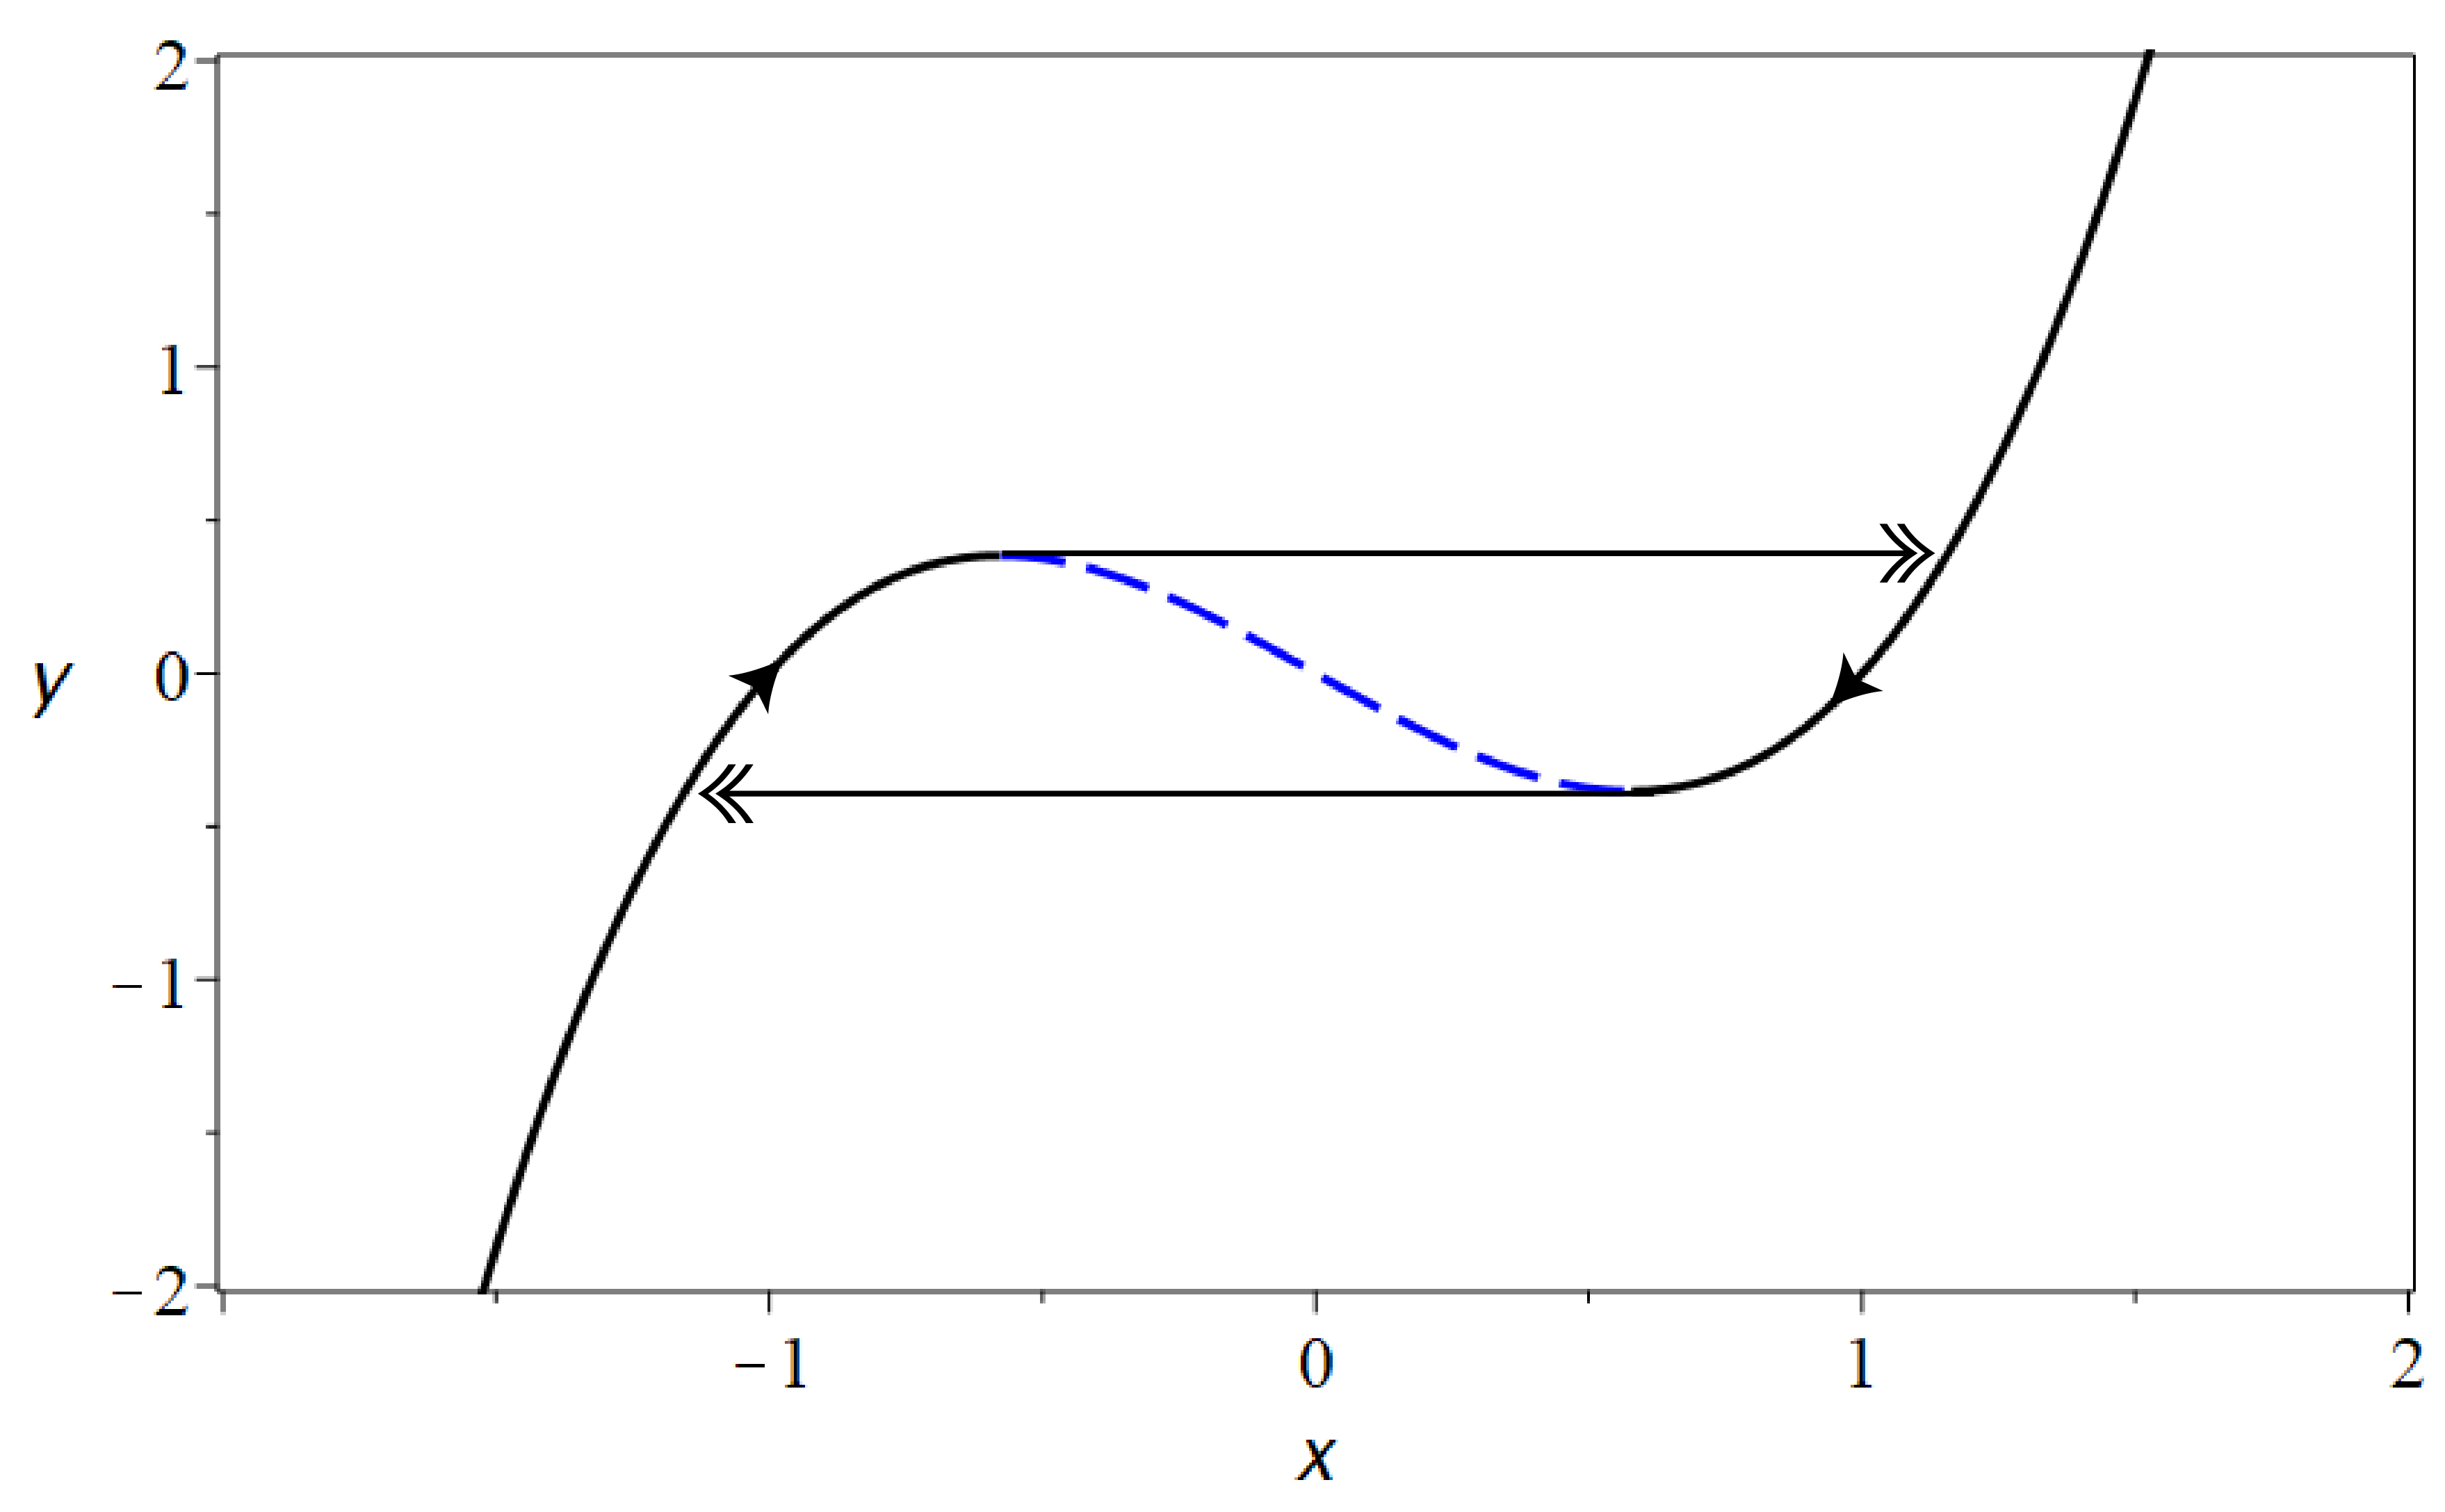
\includegraphics[width=0.8\textwidth]{slowfastcycle3}

